\chapter{Implementation Scenario}

In this chapter, I will briefly describe my implementation scenario, including the system architecture overview, system component structures as well as functionalities and communication flows. Also the implementation tool support will be introduced.
\section{Overview}
 \begin{figure}[!htb]
	\centering
	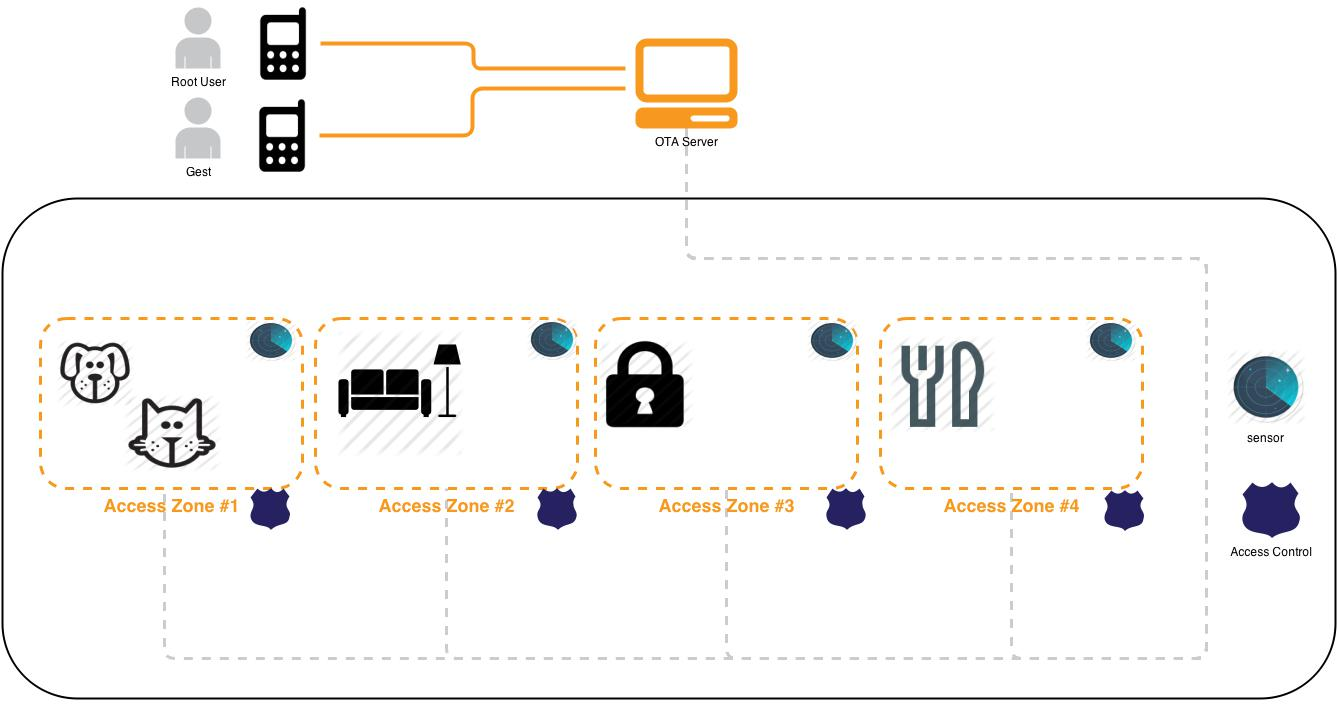
\includegraphics[width=1\textwidth]{homeoverview.jpg}
		\caption{Smart Home Scenario}
	\label{fig:SmartHome}
\end{figure}

Figure~\ref{fig:SmartHome} describes the basic structure and functionalities provided by implementation scenario  -  Smart Home. In the above-pictured automated home, following devices are introduced.
\begin{itemize}
\item Housing devices. Such as temperature sensors, coffee machine and digital door lock. They are integrated with OPC UA server application and provide house holder a comfortable and secure living condition by offering services such as:
\begin{itemize}
\item General device state query functionality.
\item Door lock access control management.
\item Home temperature and luminance management and coordination.
\item Notification and alert.
\end{itemize}
\item Smart Phone. With the help of the on smart phone installed  Android  application, \emph{Smart Home App}, which provides OPC UA client functions, the house holder is able to remotely manage housing devices.
\item Remote Administrator server  (Over The Air Server)  and smart cards. Smart cards, which are integrated in housing devices and smart phones, are installed with Java card applet \emph{CommunicationStack}, that realizes the communication stack of OPC UA architecture. The duties of smart card and remote server peers are  communication partner authentication and identification, public key management as well as  secure message transmitting.
\end{itemize}

\section {Component Structure}
 \begin{figure}[!htb]
	\centering
	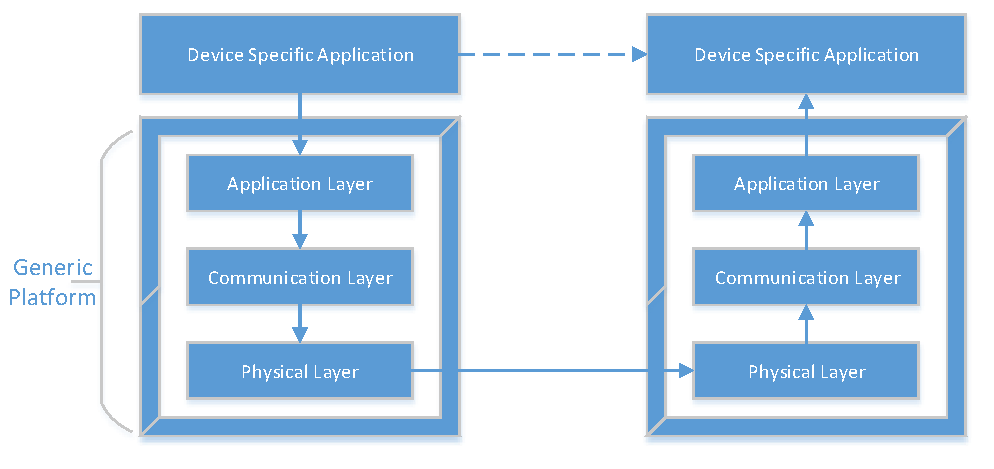
\includegraphics[width=1\textwidth]{component}
		\caption{Smart Home System Component Structure}
	\label{fig:SmartHomeComponent}
\end{figure}
With inspiration offered by application described in section~\ref{secAgent}, in order to provide a generic application platform for devices manufactured by various vendors, my demonstration Smart Home system consists of components, \footnote{Housing devices and smart phone are generically referred as Smart Home system components.} whose basic structure is illustrated in figure~\ref{fig:SmartHomeComponent}.  As can be seen, components are composed of a device specific application and a generic communication platform, which includes three layers. From bottom to top, they are:

\begin{itemize}
\item Physical layer. In this layer secure electronic devices and facilities hardwares are deployed. Alternatively lower level component could be also in this layer of higher level component.
\item Communication layer. Smart card, the on card integrated \emph{CommunicationStack} applet and corresponding remote file/application management protocols together form this layer. The main responsibility of communication layer is to create a secure communication environment for OPC UA application layer.
\item OPC UA Application layer. OPC UA client application (installed on smart phone) and OPC UA server application (installed on other homing devices) are placed in this layer and provide a common communication and connectivity interface for higher layer device specific applications. 
\end{itemize}

Moreover this component platform also emphasizes the importance of secure messaging, peer authentication as well as authorization and provides corresponding secure mechanisms, which will be discussed in upcoming paragraphs.

 \begin{figure}[!htb]
	\centering
	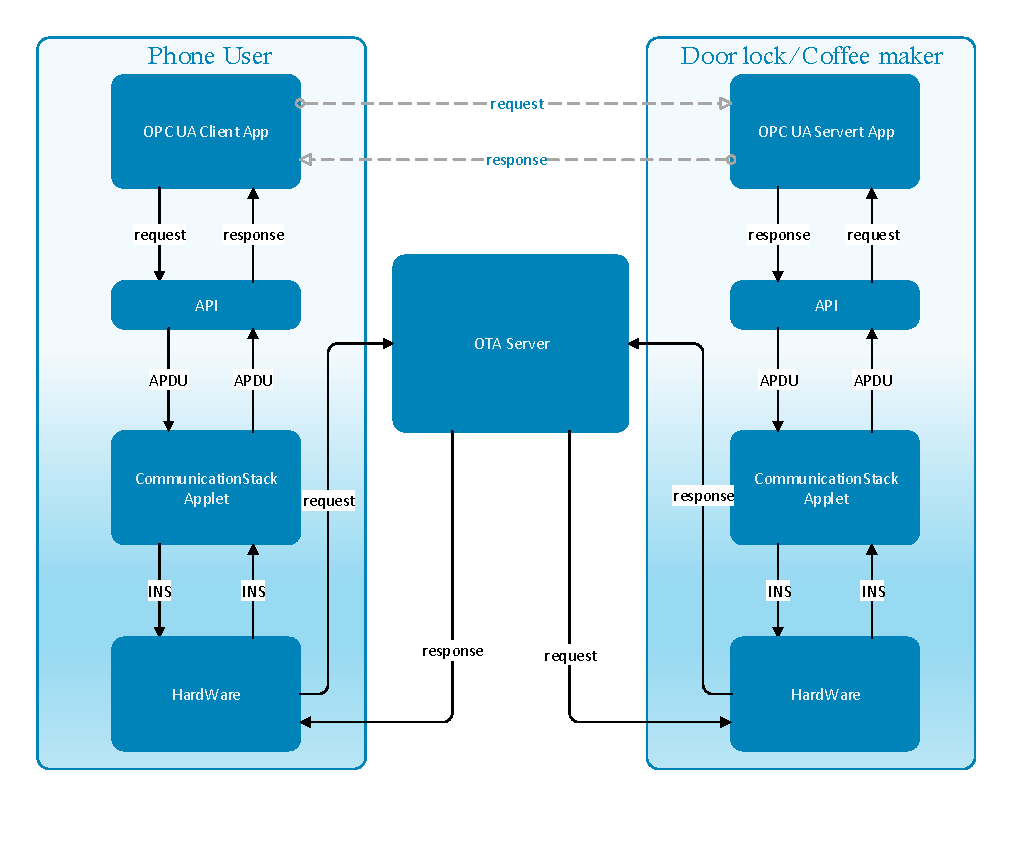
\includegraphics[width=1\textwidth]{csoverview}
		\caption{Smart Home Component Communication}
	\label{fig:softwareStructure}
\end{figure}

\section{Communication Flow}
Figure~\ref{fig:softwareStructure} pictures the communication flow between two system components.
The device hardware stands for the aforementioned component's \emph{physical layer}. \emph{CommunicationStack} together with the {internal API} construct the \emph{communication layer}.  


OPC UA client and server application communicate with each other with the help of an OTA server. And the \emph{CommunicationStack} applet is in charge of creating and managing secure communications between OTA server and secure devices. A demonstration case is given as below:

When the householder wants to make some coffee, he will send the \emph{makeCoffee} command to coffee maker with his cell phone in following steps as pictured in figure~\ref{fig:softwareStructure}. 
\begin{enumerate}
\item Phone user touches his screen and selects the \emph{makeCoffee} command. Then OPC UA client application installed on the cell phone initially generates the \emph{makeCoffee} request and forwards it to the internal API
\item The internal API translates the request into a remote APDU object and sends the APDU to the \emph{CommunicationStack} applet. Before the \emph{CommunicationStack} is able to forward the request APDU, it must create a secure communication channel with the remote server.
\item The remote server will then in this step firstly exam the identify of the message sender.
\item After a successful mutual identification, a secure channel will be established between smart phone and the remote server, the \emph{makeCoffee} request is going to be transmitted  to the remote sever with the help of this newly created secure messaging channel.
\item After receiving the command from message sender, remote server will find the correct message receiver and forward the command to him. 
\item  In the last step, the \emph{makeCoffee} command will be received by the \emph{CommunicationStack} installed in target coffee machine, whose \emph{internal API} translates the request and forwards it to the OPC UA server application. The OPC UA server application will then control the coffee maker and perform the make coffee function. Alternatively it also generates a response message and notifies the phone user that its job is successful finished. 
\end{enumerate}
The two core system parts involved in above described scenario are \emph{CommunicationStack} applet and \emph{OPC UA client/server application code} 

\subsection{CommunicationStack Applet}
\emph{CommunicationStack} is integrated in UICC smart card, whose duties are realizing secure channel as well as session management, transporting data to receiver using TCP/IP connections or SMS. To be more specifically, the \emph{CommunicationStack}'s responsibilities are:
\begin{itemize}
  \item initiate session based Http connection, which is protected by TLS 1.2 protocol  (proactive)
  \item trigger Http session based on received trigger SMS, that is proposed and send by OTA server (passive)
  \item rebuild broken communication channel
  \item message encryption as well as decryption
  \item message transmit
\end{itemize}

\subsection{OPC UA Application Functionalities}\label{secFunction}
In this paragraph, a brief introduction about functionalities offered by  the OPC UA  client and server application code is presented.

In conclusion, OPC UA server on secure housing device provides following services:
 \begin{itemize}
  \item processing client's subscription
  \item publishing notification.
  \item client authority management.
  \item historical data record.
  \item execution of client's command.
  \item managing the homing device on which the OPC UA server runs.
\end{itemize}
Basic OPC UA client functions as following are provided by smart phone applications:
 \begin{itemize}
  \item submitting subscription
  \item receiving published data from OPC UA server.
  \item sending command and configuration data.
  \item querying system historical record.
  \item providing user friendly GUI interface.
\end{itemize}


 \begin{figure}[!htb]
	\centering
	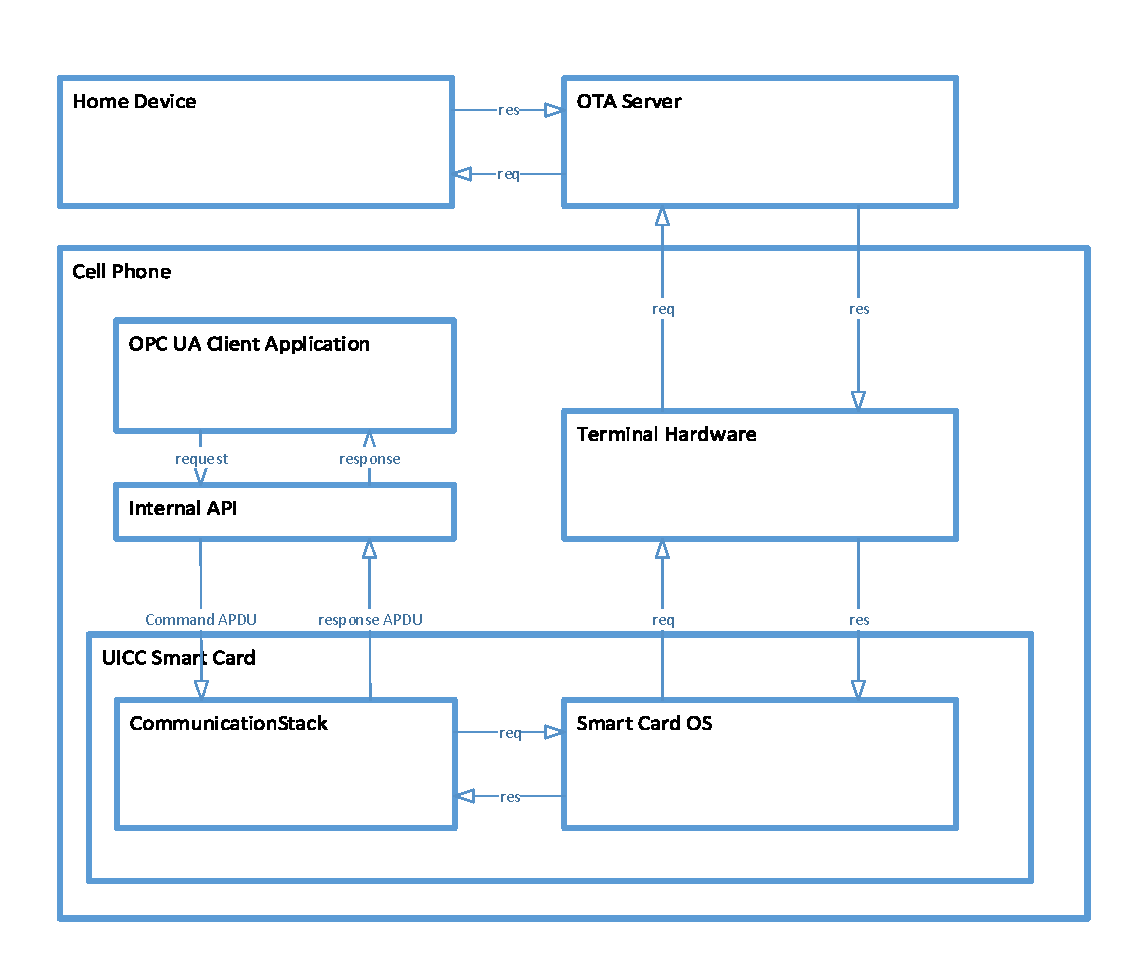
\includegraphics[width=1\textwidth]{clientStructure}
		\caption{Cell Phone Component Architecture}
	\label{fig:clientStructure}
\end{figure}

\subsection{Cell Phone Component Software Structure}
As described in figure~\ref{fig:clientStructure}, the smart phone introduced in my application scenario consists of OPC UA client application code that realizes client application level functions, internal API, \emph{CommunicationStack} applet, smart card and phone hardware.

\begin{figure}[!htb]
	\centering
	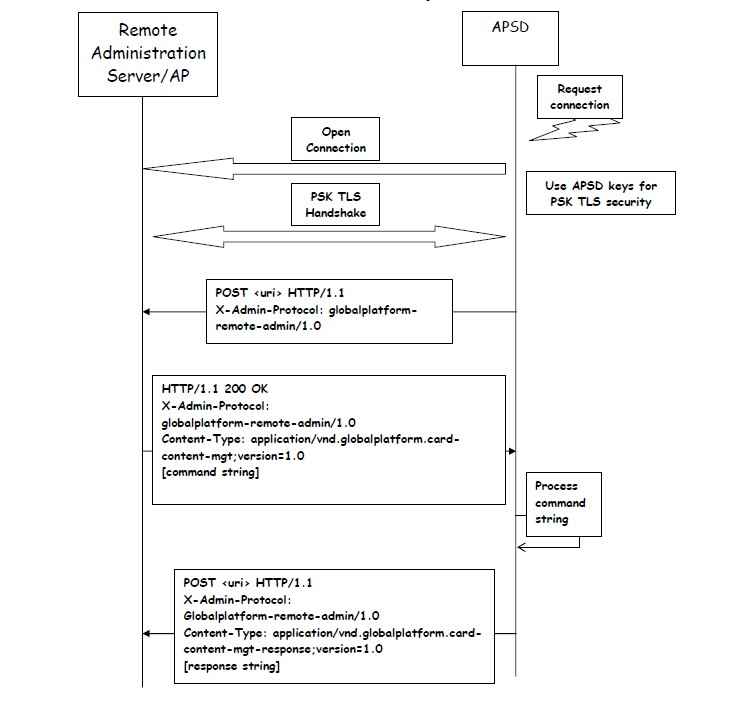
\includegraphics[width=1\textwidth]{apsd.jpg}
		\caption{Communication Flow between AP and APSD \cite{ramGP}}
	\label{fig:apsd}
\end{figure}
The remote communication flow applied in my application scenario is compliant with the one provided by GlobalPlatform as shown in figure~\ref{fig:apsd}. GlobalPlatform defines the mechanisms for secure information exchange between a remote entity and a terminal, which is also known as Remote Application/File Management(RAM/RFM) over Http protocol. 

Application Security Domain (APSD) issued by GloablPlatform represents the terminal device in the realm of RAM/RFM and the aforementioned remote entity  is also referred as Remote Administration Server. 

With these two concepts, smart card holding the appropriate Security Domain can act as a Http client and is capable of packing APDU format information into Http POST message and transmitting this Http message to the OTA server, who will forward the message to the target receiver \cite{ramGP}. Moreover in oder to protect the confidentiality and integrity of exchanged information, I proposal that a \emph{public key infrastructure} is also integrated in the OTA server, which manages the public keys of Smart Home housing devices and adds additional security protection to my system.
 
Figure~\ref{fig:apsd} illustrates a typical RAM communication flow between administration server and corresponding security domain (Application Security Domain) on smart card. As can be seen, the request for open communication channel is usually initialized by security domain, which represents the phone user. After a successful secure handshake, the remote administration server and security domain are able to based on Http connection exchange request and response strings, which encapsulate APDU instructions. GlobalPlatform has also provided  a list of APIs used to initialize authentication process, to configure cipher suits and to perform secure messaging.

\subsection{Housing Device Component Software Structure}

\begin{figure}[!htb]
	\centering
	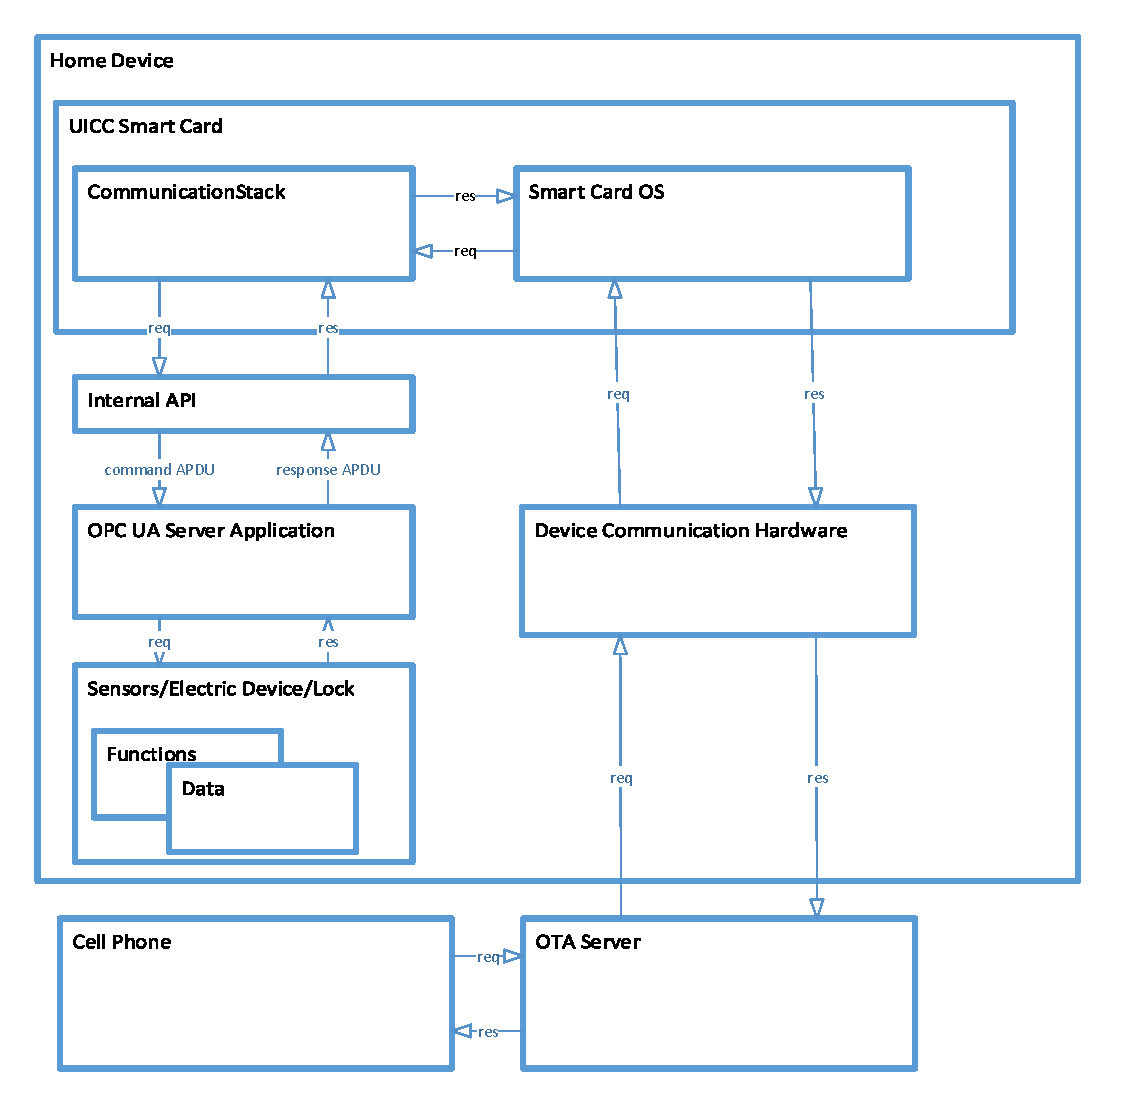
\includegraphics[width=1\textwidth]{serverStructure}
		\caption{Housing Device Component Architecture}
	\label{fig:serverStructure}
\end{figure}
Housing Device here refers to sensors, household electrical appliances as well digital locks that together build up the Smart Home system. Each secure device provides services described in section~\ref{secFunction}. The device software structure is pictured as figure~\ref{fig:serverStructure} and it consists of OPC UA server application code, which offers basic functionalities like subscription and notification mentioned before, an internal API, an on smart card integrated \emph{CommunicationStack} applet and device specific functions as well as device data.

\subsection{Implementation Tool Support} \label{secTS}
In this paragraph, I will shortly present the tools that I applied to design, program and test my Smart Home demonstrating system.
\subsubsection{Java Card Application Design and Debug Tool}
Morpho presents JACADE with full name, Java Card Applet Develop Environment, which is more than just a IDE but a complex selection of various class APIs and software modules, that can be applied to design complete Java Card applet as well as to debug Java Card source. 
\subsubsection{Java Card Applet Testing Environment}
When it comes to running test with Java Card applet, tester has two options. Firstly, he can install the to be tested applet on a smart card and then connect this chip card with test computer using \emph{Morpho Card Reader (MCR)}. Alternatively \emph{Java virtual card} which is integrated with the to be tested applet  could be also applied. 

In either way, as next step \emph{Universal Test Environment (UTE)} will be applied. \emph{UTE} presented and developed by Morpho uses Java language developed test cases
 and test scenarios\footnote{Test scenario is a collection of relative test cases.} to simulate desired use cases and observes corresponding smart card reactions. With the observed test result, tester will be able to analyze applet performance and debug corresponding application code. For instance \emph{UTE} can integrate software models used to simulate security domain standardized by \emph{Globalplatform} and perform the sophisticated user authentication process.
\subsubsection{Android Application Design Tool}
Eclipse IDE for Java Developer of version 3.7.1, together with Android SDK \emph{seek-for-android} and ADT plug-in, are applied as Android application development environment. Moreover Android of version 2.3.5 is simulated and chosen as platform for the \emph{Smart Home App}.
\subsubsection{Smart Home Simulation Environment}
In order to simulate the data managed by home electronic device, \emph{MySQL} database is employed. And together with \emph{PHP of version 5.5.12}, \emph{Apache of version 2.4.9}, the web server for Smart Home is created. Android application \emph{Smart Home App} communicates with this web server for the purpose of scenario testing and demonstration.

\section{Conclusion}
In this chapter, I briefly described the concept of my demonstration scenario and discussed the system components architecture as well as adapted communication flow. Moreover the supporting programming and testing tools are also presented. In the next chapter, I will detailedly describe how I design my \emph{CommunicationStack} applet, \emph{Smart Home App} and the Smart Home web application.